\documentclass[12pt,letterpaper]{book}

\usepackage{xcolor}

\usepackage{tocstyle}
\usetocstyle{standard}


\renewcommand{\today}{February 26-28, 2020}

\usepackage[a4paper,margin=3cm,innermargin=3cm]{geometry}

\usepackage[
 type={CC},
 modifier={by-nc-nd},
 version={4.0},
]{doclicense} 

\usepackage{needspace}
\usepackage{marginnote}
\usepackage{ifxetex}
\renewcommand*{\marginfont}{\sffamily\footnotesize}

\usepackage{imakeidx}

\usepackage[hidelinks]{hyperref}
\hypersetup{
pdftitle={Book of Abstracts},
pdfsubject={WFM2020},
pdfauthor={Patrick Diehl},
pdfkeywords={phase fields,peridynamics,experimental mechanics}
}
\makeindex[intoc]

\newenvironment{conf-abstract}[4][]{
 \needspace{10\baselineskip}
 \begin{center}
 { \renewcommand\textsuperscript[1]{}
 \phantomsection\addcontentsline{toc}{section}
 {\texorpdfstring{#2 (\emph{#3})}{#2 (#3)}}
 }
 {{\large\bfseries #2}\marginnote{#1}\par}
 \medskip
 {#3\par}
 \smallskip
 {\small #4\par}
 \end{center}
}{%
 \bigskip
 \hrule
 \bigskip
}

\usepackage{etoolbox}
\newcommand{\indexauthors}[1]{%
 \forcsvlist{\index}{#1}
}

\setcounter{tocdepth}{3}
\setcounter{secnumdepth}{-1}
\pagestyle{plain}


\title{USACM Thematic Workshop on Experimental and Computational Fracture Mechanics: \\
	\large Validating peridynamics and phase field models for fracture prediction and experimental design}
\author{Venue: \\ Center of Computation \& Technology \\ Louisiana State University}

\ifxetex
\usepackage{fontspec}
\setmainfont{Raleway}
\fi

\usepackage{timetable/calendar} 

\usepackage{rotating}

\usepackage{datatool}

\DTLloaddb{data}{./data.csv}
\DTLloaddb{dataPoster}{./dataPoster.csv}


\newcommand*{\thevalue}{}
\newcommand*{\getCol}[2]{%
 \DTLgetvalueforkey{\thevalue}{Last}{data}{Talk}{#2}%
}

\newcommand*{\lastname}[2]{
\getCol{1}{#1}
\thevalue 
}


\newcommand*{\thevalues}{}
\newcommand*{\getCols}[2]{%
 \DTLgetvalueforkey{\thevalues}{Time}{data}{Talk}{#2}%
}



\newcommand*{\gettime}[2]{
\getCols{1}{#1}
\kern-1ex\thevalues
}



\begin{document}

\frontmatter

\maketitle

This workshop is sponsored by

\begin{itemize}
\item Technical Thrust Area on Large Scale Structural Systems and Optimal Design of the US Association for Computational Mechanics
\item Louisiana State University Center for Computation \& Technology 
\item Oak Ridge National Laboratory
\item Society for Experimental Mechanics
\item U.S. National Committee on Theoretical and Applied Mechanics (AmeriMech)
\end{itemize}

\newpage

\section*{Abstract}
The comparison against experimental results is essential to validate models and discretizations in order to gain confidence in the approach’s predictability and reliability. Peridynamics and phase field methods have been utilized for fitting or validation against experimental results. When using experimental results. the question arises if the experimental data is mature enough to provide all data to set up the simulations, e.g. applied loading, and compare the experimentally measured quantity of interest with the one obtained by simulation. \\

During this workshop the phase field and peridyanmic community showcases which kind of experiments were used for validation and the difficulties phased. The experimental fracture mechanics community emphasizes the experiments they are researching on and what kind of simulations would be interesting for them to gain more understanding of experimental phenomena observed. \\

This workshop brings together experts on experimental fracture mechanics and experts in modelling and simulating crack and fractures utilizing peridyanmic and phase fields methods. As a results, it will elaborate the collaboration between the three participating communities and starts the discussion about a set of experiments used as a benchmark problem for a robust validation of phase field and peridyanmic models.

\section*{Organization committee }
\begin{itemize}
\item Patrick Diehl, Louisiana State University
\item Pablo Seleson, Oak Ridge National Lab
\item Serge Prudhomme, Ecole de Polytechnique Montreal
\end{itemize}

\section*{Scientific committee}
\begin{itemize}
\item Stuart Silling, Sandia National Lab
\item Robert Lipton, Louisiana State University
\item John Dolbow, Duke University
\item K. Ravi-Chandar, The University of Texas at Austin
\item Yuri Bazilevs, Brown University 
\end{itemize}


\chapter{Welcome Address}
Welcome\\\newline
\noindent
It is my distinct pleasure to welcome you all to the Workshop on Experimental and Computational Fracture Mechanics (February 26-28, 2020) held at the Center for Computation and Technology (CCT) on the Louisiana State University campus in Baton Rouge, Louisiana.\\\newline
\noindent
I am pleased to be able to support and co-sponsor this workshop with a number of others: The Technical Thrust Area on Large Scale Structural Systems and Optimal Design of the US Association for Computational Mechanics, the Oak Ridge National Laboratory, the Society for Experimental Mechanics, and the U.S. National Committee on Theoretical and Applied Mechanics (USNC/TAM). We at CCT greatly appreciate the support of our co-sponsors. In addition, I would like to thank the great work of the organizers of this workshop, Dr. Patrick Diehl, Dr. Serge Prudhomme, and Dr. Pablo Seleson.\\\newline
\noindent
This workshop brings together experts in experimental fracture mechanics, peridynamics, and phase field methods to discuss the state-of-the-art of experimental measurement and computational modeling with applications in fracture mechanics. We hope this will promote dialogue between these communities, and help to identify challenges and pathways for robust validation of phase field and peridynamic models as well as the integration of experimental and modeling efforts.\\\newline
\noindent
I would like thank the three excellent keynote speakers, Dr. Stewart Silling (Sandia Labs), Prof. Lallit Anand (MIT), and Prof. K. Ravi-Chandar (UT Austin), who are world-class experts in peridynamics, phase field, and experimental fracture mechanics, for sharing their thoughts on the field. In addition, I thank all the participants of the event.\\\newline
\noindent
I sincerely hope you enjoy and benefit from this unique workshop and the discussion sessions during the coming two and a half days.\\\newline
\noindent
With best wishes,\\\newline
\noindent
J. “Ram” Ramanujam


%\begin{sidewaysfigure}
%\begin{calendar}{\textwidth} % Calendar to be the entire width of the page

\setcounter{calendardate}{23} % Day on which the calendar starts - note that you have to account for blank days

%----------------------------------------------------------------------------------------
%	Monday
%----------------------------------------------------------------------------------------

\day{}{}

%----------------------------------------------------------------------------------------
%	SECOND DAY
%----------------------------------------------------------------------------------------

\day{}{}

%----------------------------------------------------------------------------------------
%	THIRD DAY
%----------------------------------------------------------------------------------------

\day{Arrival}{
\textbf{Reception} The Cook Hotel (7:00-9:00) \\\daysep
}
%----------------------------------------------------------------------------------------
%	FOURTH DAY
%----------------------------------------------------------------------------------------


\day{Day 1}{
\textbf{Registration/Coffee} (8:15-8:45) \\\daysep
Welcoming Remarks (8:45-9:00)\\\daysep
\lastname{1}~ (9:00-10:00) \\\daysep
\textbf{Coffee Break} (10:00-10:30) \\\daysep
\lastname{2}~ (10:30-11:00) \\\daysep
\lastname{3}~ (11:00-11:30) \\\daysep
\lastname{4}~ (11:30-12:00) \\\daysep
\lastname{5}~ (12:00-12:30) \\\daysep
\textbf{Lunch} (12:30-14:00) \\\daysep
\lastname{6}~ (14:00-14:30) \\\daysep
\lastname{7}~ (14:30-15:00) \\\daysep
\lastname{8}~ (15:00-15:30) \\\daysep
\textit{Discussion }  (15:30-16:00) \\\daysep
\textbf{Coffee Break} (16:00-16:30) \\\daysep
\lastname{9}~ (16:30-17:00) \\\daysep
\lastname{10}~ (17:00-17:30) \\\daysep
}

%----------------------------------------------------------------------------------------
%	FIFTH DAY
%----------------------------------------------------------------------------------------

\day{Day 2}{
\textbf{Registration/Coffee} (8:30-9:00) \\\daysep
\lastname{11}~ (9:00-10:00) \\\daysep
\textbf{Coffee Break} (10:00-10:30) \\\daysep
\lastname{12}~ (10:30-11:00) \\\daysep
\lastname{13}~ (11:00-11:30) \\\daysep
\lastname{14}~ (11:30-12:00) \\\daysep
\lastname{15}~ (12:00-12:30) \\\daysep
\textbf{Lunch} (12:30-14:00) \\\daysep
\lastname{16}~ (14:00-14:30) \\\daysep
\lastname{17}~ (14:30-15:00) \\\daysep
\textit{Discussion} (15:00-15:30) \\\daysep
\textbf{Coffee Break}~ (15:30-16:00) \\\daysep
\lastname{18}~ (16:00-17:00) \\\daysep
\lastname{19}~ (17:00-17:30) \\\daysep
\textbf{Banquet} Faculty Club LSU (19:00-21:00)\\
}

%----------------------------------------------------------------------------------------
%	SIXTH DAY
%----------------------------------------------------------------------------------------


\day{Day 3}{
\textbf{Registration/Coffee} (8:30-9:00) \\\daysep
\lastname{20}~ (9:00-09:30) \\\daysep
\lastname{21}~ (9:30-10:00) \\\daysep
\textbf{Coffee Break}~ (10:00-10:30) \\\daysep
\lastname{22}~ (10:30-11:00) \\\daysep
\lastname{23}~ (11:00-11:30) \\\daysep
\lastname{24}~ (11:30-12:00) \\\daysep
General discussion (12:00--12:30) \\\daysep
\textbf{Lunch} (12:30-14:00) \\\daysep
}



%----------------------------------------------------------------------------------------
%	SEVENTH DAY
%----------------------------------------------------------------------------------------





% Note: more days can be added to give the calendar a third or fourth week

%----------------------------------------------------------------------------------------

\finishCalendar
\end{calendar}
%\end{sidewaysfigure}

\newpage

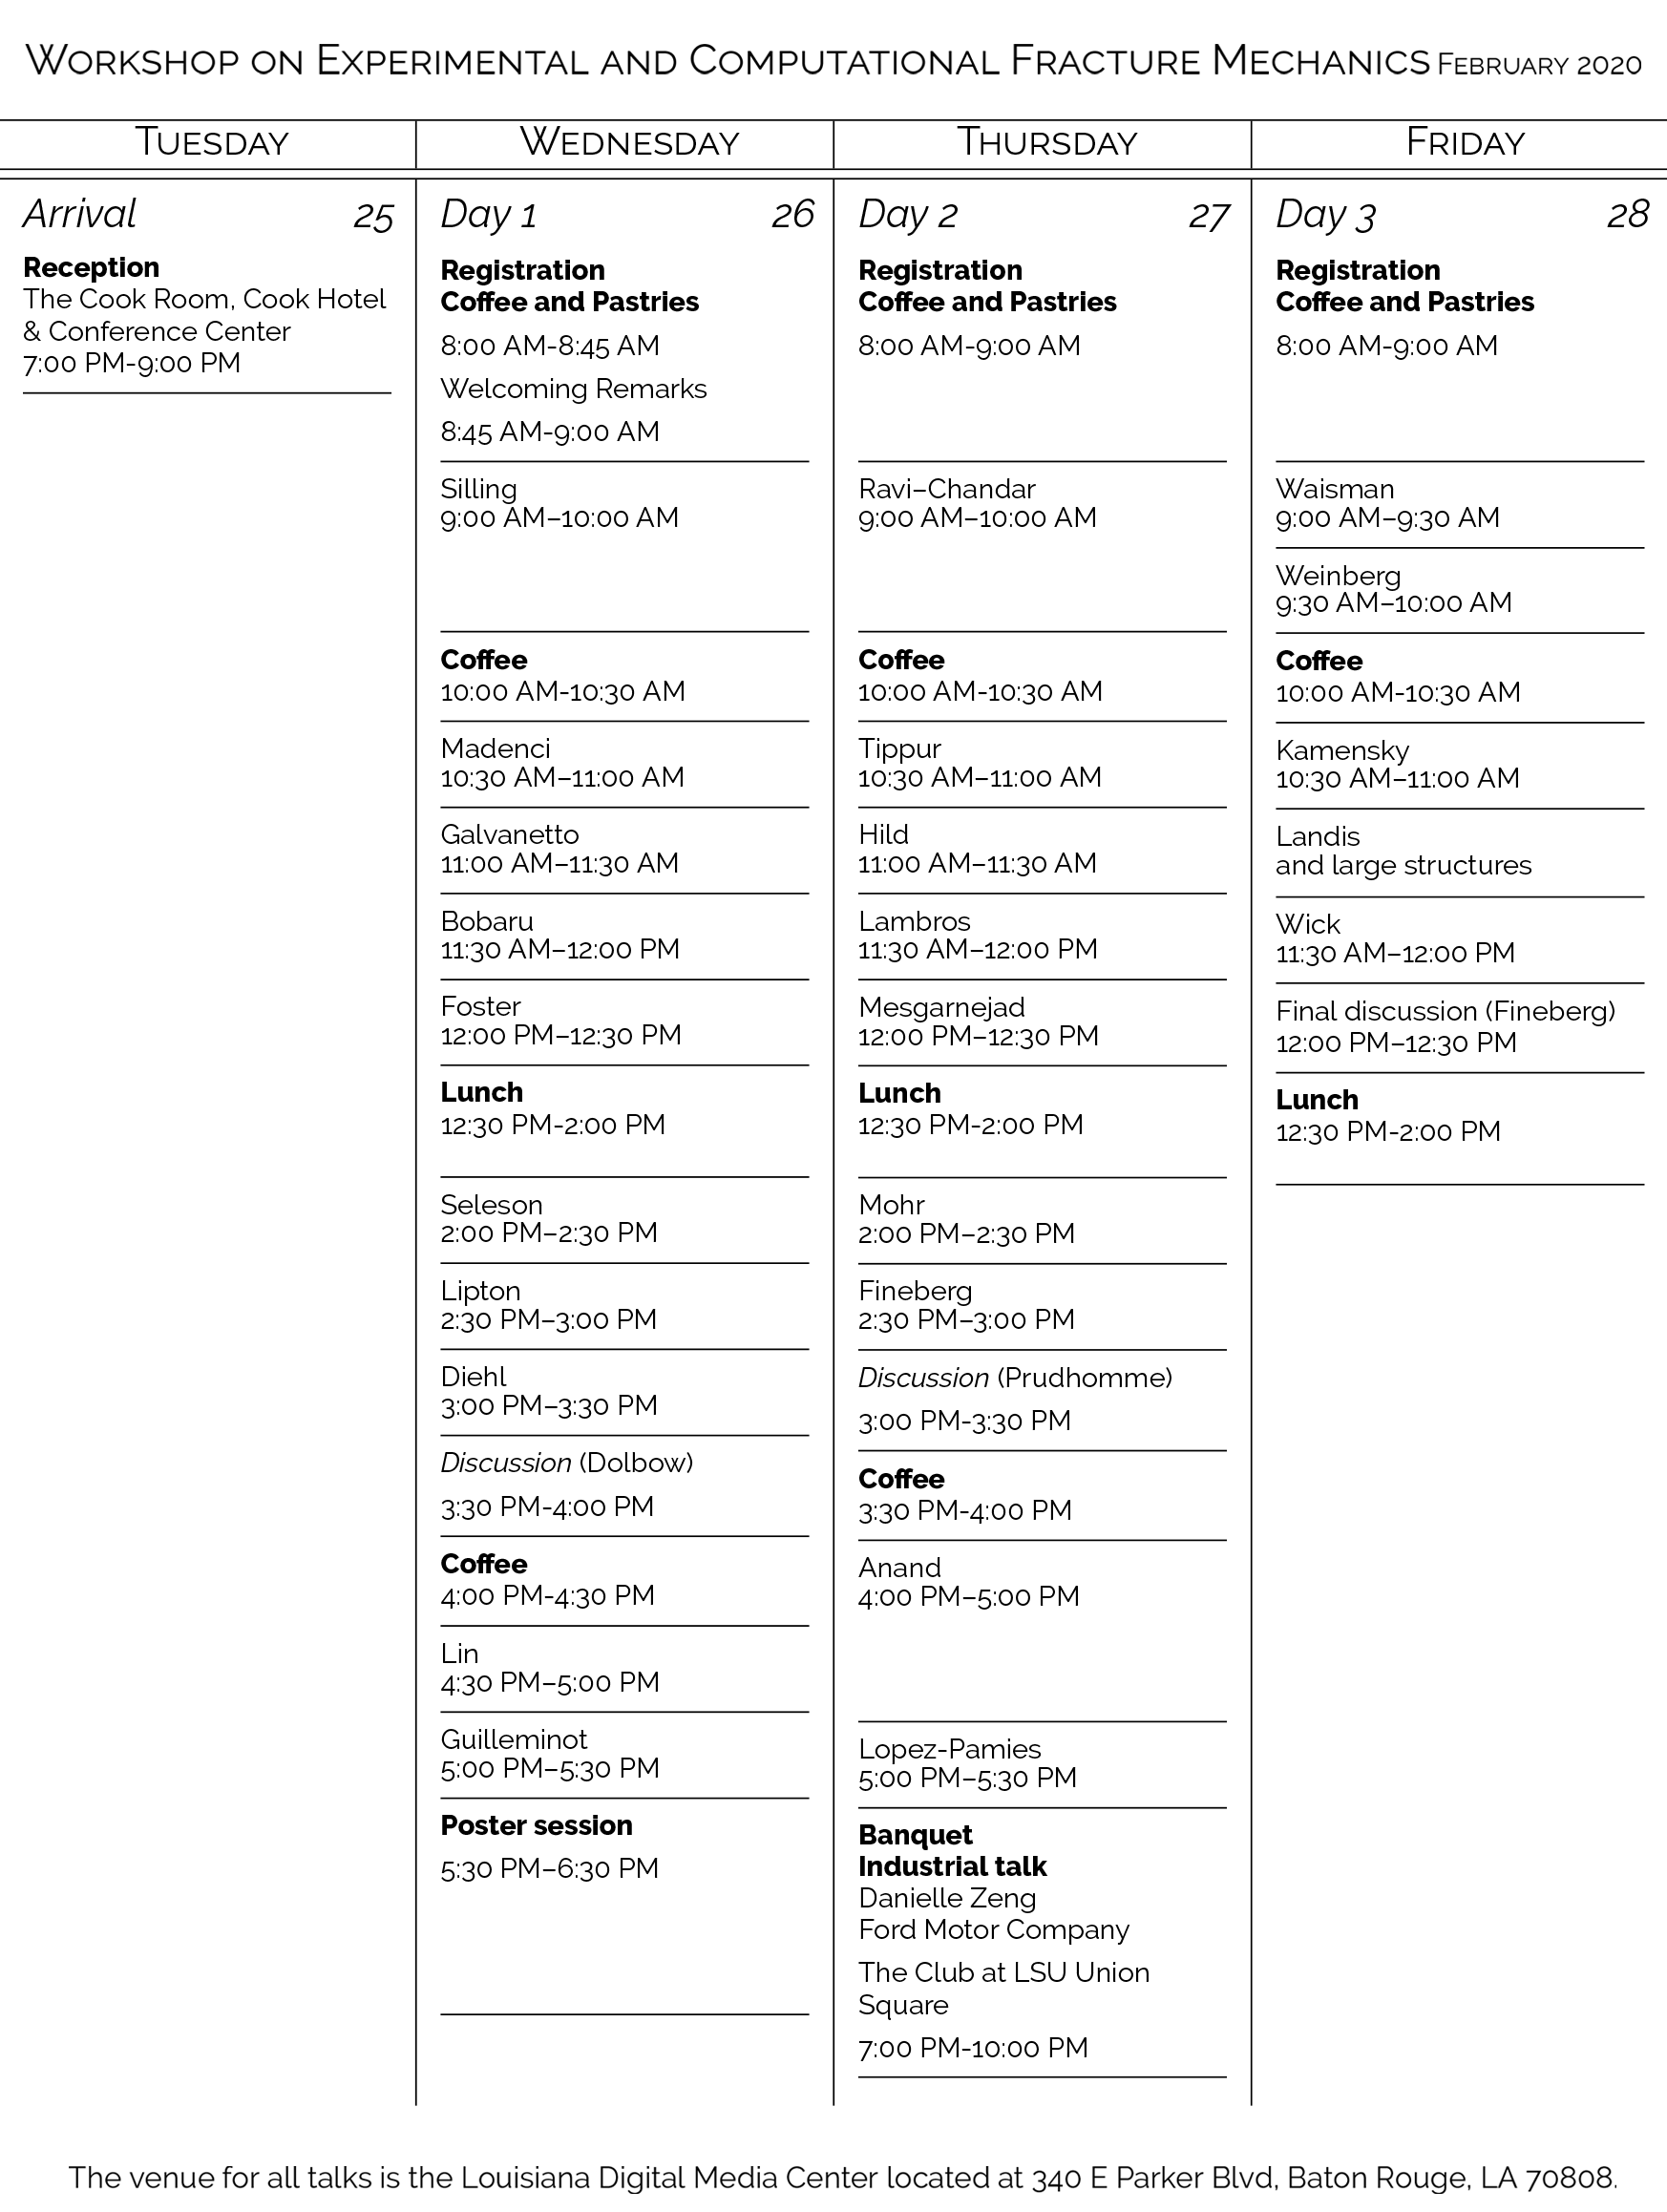
\includegraphics[width=\linewidth]{timetable_edit.png}


\tableofcontents

\mainmatter

\chapter{Industrial talk}

\begin{conf-abstract}[27$^{th}$]
{Integrated Computational Materials Engineering (ICME) development of carbon fiber composites for lightweight vehicles}
{Danielle Zeng}
{Ford Motor Company}
\index{Zeng~Danielle}
\begin{center}
\textit{Co-Authors: Pablo Seleson, Bo Ren, and C.T. Wu}
\end{center}
Automotive manufacturers use lightweight materials to meet the increasing demands of fue l efficiency. The Carbon Fiber Reinforced Polymer (CFRP) composites, with a density of 1.55 g/cm3 and a tensile strength of 2000 MPa in the fiber direction, are among the most promising candidate s to replace the metals currently used for structural components. It is important to note that the performance of carbon fiber composites is determined not only by the component design, but also the manufacturing processes. In this talk, the focus is on the application of an Integrated Computational Materials Engineering (ICME) approach to the structural composite design. A suite of predictive models is developed to link materials design, manufacturing process and final performance to enable optimal design and manufacturing of CFRP components for automotive vehicles.

One of the greatest challenges for successfully applying the ICME approach to CF composites is how to accurately simulate the different failure modes during crash scenarios. Especially, the traditiona l thin shell model in finite element simulation has difficulty in capturing the delamination behavior during complex loading conditions. Recently, a discontinuous Galerkin weak form for bond-based peridynamic models is developed for composite modeling through the collaboration among ORNL, LSTC and Ford. The accuracy and computational efficiency of the developed model for delamination modeling is demonstrated through simulating a dynamic bending test of a laminate structure.
\end{conf-abstract}


\chapter{Talks}

\DTLforeach*{data}{\last=Last,\first=First,\affiliation=Affiliation,\title=Title,\datum=Date,\time=Time,\text=Abstract}
{
\begin{conf-abstract}[\datum\\\tiny\time]
{\title}
{\first~ \last}
{\affiliation}
\indexauthors{\last~\first}
\input{\text}
\newpage
\end{conf-abstract}
}

\chapter{Posters}

\DTLforeach*{dataPoster}{\last=Last,\first=First,\affiliation=Affiliation,\title=Title,\datum=Date,\time=Time,\text=Abstract}
{
\def\x{\last}
\def\y{\substring{\x}{1}{1}\par}
\begin{conf-abstract}[\datum\\\time]
{\title}
{\first~\last}
{\affiliation}
\indexauthors{\last~\first}
\begin{center}
\input{\text}
\end{center}
\end{conf-abstract}
}


% Specify conf-abstract like this:
% \begin{conf-abstract}[optional text going into the margin note]
% {Title of Paper}
% {Authors (use \textsuperscript as institution markers)}
% {Institutions (use \textsuperscript as institution markers)}
% \indexauthors{Lastname1!Firstname 1, Lastname2!Firstname2}
% Abstract text
% \end{conf-abstract}
%
% It's probably best to generate the abstracts from a 
% database or something via a script. Don't forget to
% check through for any special characters that need to
% be escaped.

%\input{abstracts/paper1}
%\input{abstracts/paper2}
%\input{abstracts/paper3}

\chapter{Additional information}

\section{Addresses}

\subsection*{Workshop venue}
Digital Media Center, Center for Computation \& Technology, 340 E Parker Blvd., Baton Rouge, LA 70803
\subsection*{Hotel}
The Cook Hotel at LSU, 3848 W Lakeshore Dr, Baton Rouge, LA 70808 \\
(225) 383-2665
\subsection*{Banquet}
LSU Faculty Club, 101 Tower Dr, Baton Rouge, LA 70803 \\
(225) 578-2356

\section{Restaurants}

\subsection*{Walking distance}

\begin{itemize}
\item The Chimes -- Lively campus-area hangout from a local chain featuring a worldwide beer list \& hearty bar fare: 3357 Highland Rd, Baton Rouge, LA 70802 (225 383-1754)
\item Louie's Cafe -- LSU-area fixture dating to 1941 serves a diner menu 24/7 in a classic lunch-counter setting: 3322 Lake St, Baton Rouge, LA 70802 (225 346-8221)
\item Highland Coffees -- Charming, airy locale with a laid-back vibe for coffee roasted on-site \& a variety of baked goods: 3350 Highland Rd, Baton Rouge, LA 70802 (225 336-9773)
\end{itemize}

\subsection*{Local cuisine}

\begin{itemize}
\item Parrain's Seafood Restaurant -- Local seafood specialist cooking up Louisiana recipes in a rustic space with porch seating: 3225 Perkins Rd, Baton Rouge, LA 70808 (225 381-9922)
\item Mike Anderson's - Baton Rouge -- Area staple for regional seafood in a spacious, wood-lined setting with a sports-friendly vibe: 1031 W Lee Dr, Baton Rouge, LA 70820 (225 766-7823)
\item Stroubes Seafood and Steaks -- Chophouse presenting local preparations of meat \& seafood in comfortable digs with a lounge: 107 3rd St, Baton Rouge, LA 70801 (225 448-2830)
\end{itemize}


\backmatter
\renewcommand{\indexname}{Author Index}
\printindex
\newpage
\doclicenseThis 

\end{document}
